\chapter{Kubernetes}

Kubernetes is one of the most widely used container orchestration tools. Many cloud platforms provide Kubernetes support. Many opponent container orchestration tools are built on top of Kubernetes.

\section{Kubernetes Basics}

\mync{Kubernetes}, also known as \mync{k8s}, is an open-source container orchestration system originally developed by Google. It automates the deployment, scaling, and management of containerized applications.

As a orchestration tool, Kubernetes mainly focuses on the following items:
\begin{itemize}
	\item Monitor the status of the containers, and restart / replace broken ones.
	\item Balance the load among containers.
	\item Scale up and down the number of containers based on the total load.
\end{itemize}
From the above, Kubernetes can be seen as a more powerful practice of what docker compose tries to do. It comes with additional features such as support on multi-server deployment.

Managed services such as ECS can also do container orchestration. However, these managed services are often proprietary and inclusive to a particular cloud service provider, making it difficult to migrate the containerized applications across platforms. Kubernetes, on the other hand, is open-source and platform-independent, hence would not pose that problem.

Nowadays, many cloud service providers also support Kubernetes-based container deployment, such as \myabb{Elastic Kubernetes Service}{EKS} by AWS and \myabb{Google Kubernetes Engine}{GKE} by Google Cloud. Notice that these managed services often come with some unique features built on top of Kubernetes, making the using of Kubernetes on these platform not entirely the same as (often easier than) doing it on a local machine.

\begin{shortbox}
	\Boxhead{Kubernetes and Docker Engine}
	
	Kubernetes as a container orchestration tool used to be built on top of docker engine. It used a special program \verb|dockershim| to talk to the underlying docker engine.
	
	Recently, docker support has been deprecated in Kubernetes. Consequently, \verb|dockershim| has also been removed.
\end{shortbox}


\subsection{Infrastructure}

Figure \ref{ch:vac:fig:kubernetescluster} demonstrates the key components Kubernetes has inside its cluster.
\begin{figure}[!htb]
	\centering
	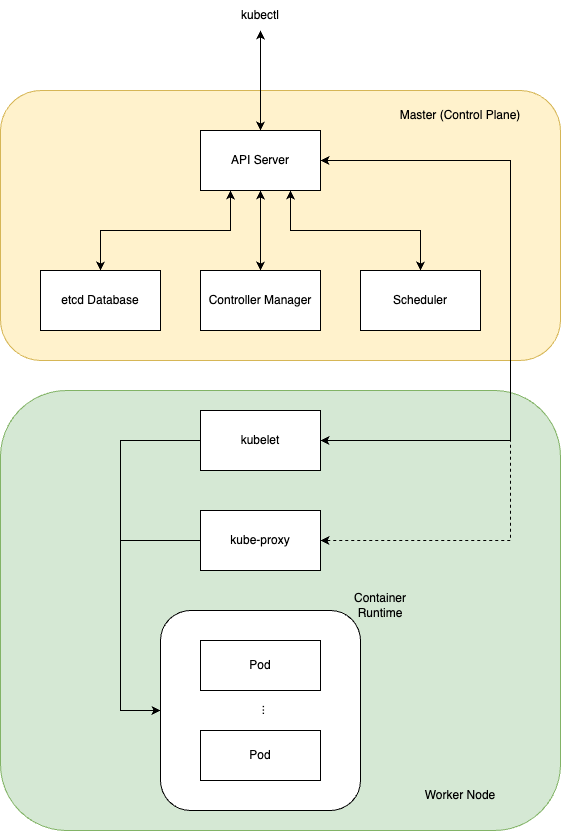
\includegraphics[width=250pt]{chapters/part-3/figures/k8sarchitecture.png}
	\caption{Kubernetes cluster and its key components.} \label{ch:vac:fig:kubernetescluster}
\end{figure}

As shown in Fig. \ref{ch:vac:fig:kubernetescluster}, Kubernetes manages containers in a centralized ``master-worker'' manner, where the master in yellow (also known as the control plane) interact with the user as well calculates the number of pods to be deployed for each work node. The work nodes in green, on the other hand, process the application data. The arrows in Fig. \ref{ch:vac:fig:kubernetescluster} represents the control flow. Notice that the application data flows differently and it does not pass through the master.

Key components in the master and the nodes and their functions are summarized in Table \ref{ch:vac:tab:keycomponents}.

\begin{table}[!htb]
	\centering
	\caption{Key components in Kubernetes master and nodes.} \label{ch:vac:tab:keycomponents}
	\begin{tabularx}{\textwidth}{llX}
		\hline
		Component & Location & Description \\
		\hline
		\verb|etcd| & Master & A distributed key-value pair database that stores the status of the Kubernetes cluster. The consistency of the distributed database is achieved based on Raft consensus algorithm. \\ \hline
		API server & Master & The gateway to handle all interactions with the Kubernetes cluster. For example, \textit{kubectl} requests from the user are handled by API server. \\ \hline
		Scheduler & Master & The optimizer that calculates the desired pod distributions among all nodes based on the total load and the hardware limits. Notice that scheduler is not involved into load balance directly. A separate load balancer service can be created to actually direct the traffic. \\ \hline
		Controller Manager & Master & A set of controllers or control functions to reconcile the actual Kubernetes cluster status with what has been calculated by the scheduler and stored in \verb|etcd|. \\ \hline
		Kubelet & Node & Local controller for the node. It ensures that all the pods assigned to the node are running, and it keeps listening to the master for further instructions. \\ \hline
		Kube Proxy & Node & The internet service provider in the node. \\
		\hline
	\end{tabularx}
\end{table}

It is worth mentioning that many services, such as ClusterIP, NodePort, LoadBalancer and Ingress Controllers, though being cluster-level services, run in worker nodes, not in the master. 

Each node can host multiple pods. Inside each pod is a container or a group of containers that work together closely (dependently, in many cases). Notice that in Kubernetes, containers never run directly in a node. They are always grouped into pods. A pod should be the minimal unit  that can deliver a basic function.

Both master and nodes can run on multiple servers or VMs. For master, multiple master replicas can run in parallel to take care of user requests and provide database services. The ``decision makers'', i.e. the controller manager and scheduler, run only on one of the master nodes which is elected via a leader election process. Should the decision maker master fail, one of the other masters will be promoted. For nodes, multiple nodes can run together to precess information in parallel and Kubernetes manages the distribution of load among them.

\subsection{Installation}

It is worth mentioning in the beginning that Kubernetes is not a single software. It is a concept or an architecture that involves many pieces of software, including at least:
\begin{itemize}
  \item \verb|kubectl| the CLI
  \item \verb|kube-apiserver| the API server
  \item \verb|etcd| the distributed key-value pair database
  \item \verb|kube-scheduler| the scheduler
  \item \verb|kube-controller-manager| the control manager
  \item Kubelet
  \item Kube Proxy
  \item Kubernetes-supported container runtime such as \verb|containerd|
  \item Container Network Interface (CNI) plugin such as Calico
  \item Many more tools
\end{itemize}
The installation guidance of Kubernetes can be found at its official website \textit{kubernetes.io}. In a production environment, the administrator shall install and configure the above tools on the servers by himself. This gives him the flexibility of customizing the tools. However, the process can be tedious and requires experience.

In this notebook, for demonstration purpose, we will use Minikube to help build a Kubernetes cluster. Minikube is an open-source software developed by the Kubernetes community to start a VM and run a single-node Kubernetes cluster on a local machine. It automates most of the tools installation and configuration, and it is just enough for the scope of this notebook. 

We will only install \textit{kubectl} and Minikube. As introduced earlier, \textit{kubectl} is used to interact with Kubernetes clusters deployed either locally or remotely. It is always recommended to have \textit{kubectl} installed on the local machine. The installation of \textit{kubectl} can be found at Kubernetes website at
\begin{lstlisting}
https://kubernetes.io/docs/tasks/tools/install-kubectl-linux/
\end{lstlisting}
Minikube installation can be found at
\begin{lstlisting}
https://minikube.sigs.k8s.io/docs/start/
\end{lstlisting}

Once Minikube is installed, start it using
\begin{lstlisting}
$ minikube start
\end{lstlisting}
When starting Minikube, it automatically detects which container engine to use, and some configurations might be required subsequently. For example, if it decides to use podman, it may require the user who started Minikube to be added to the sudoer list that can start podman without sudo password authentication. This can be done by editing the following file
\begin{lstlisting}
$ sudo visudo
\end{lstlisting}
with
\begin{lstlisting}
<user name> ALL=(ALL) NOPASSWD: /usr/bin/podman
\end{lstlisting}
appended to the file.

Once Minikube is started, use the following command to verify that \textit{kubectl} has detected and connected with the Kubernetes runtime.
\begin{lstlisting}
$ kubectl cluster-info
Kubernetes control plane is running at https://192.168.49.2:8443
CoreDNS is running at https://192.168.49.2:8443/api/v1/namespaces/kube-system/services/kube-dns:dns/proxy
\end{lstlisting}

\begin{shortbox}
\Boxhead{Minikube's Built-in \textit{kubectl}}

Minikube also comes with a built-in \textit{kubectl}. It is possible to use that \textit{kubectl} instead of installing one separately. To very the existence of the built-in \textit{kubectl}, start Minikube first and then use

\begin{lstlisting}
$ minikube kubectl -- cluster-info
Kubernetes control plane is running at https://192.168.49.2:8443
CoreDNS is running at https://192.168.49.2:8443/api/v1/namespaces/kube-system/services/kube-dns:dns/proxy
\end{lstlisting}
where \verb|--| in the command tells the shell that all the followed arguments shall be passed to \textit{kubectl}, but not \verb|minikube|. For convenience, one may want to use alias as follows
\begin{lstlisting}
$ alias kubectl="minikube kubectl --"
\end{lstlisting}

Although with the above been said, it is still recommended that \textit{kubectl} to be installed on the local machine, not just in the VM. 
\end{shortbox}

It is possible to run Kubernetes cluster directly on a host machine OS without VM if that machine is running Linux. However, this is not recommended for reasons pertaining to access control, security, and isolation. It is generally a better practice to deploy Kubernetes clusters in VMs.

The configuration file for \textit{kubectl} is usually located at \verb|~/.kube/config|. It determines the basic setups of the \textit{kubectl} instance, such as which Kubernetes cluster \textit{kubectl} communicates with.

\subsection{Kubernetes Cluster Configuration}

Kubernetes configuration files are used to guide Kubernetes on how it should configure the cluster and run the applications. There are often multiple configuration files in an application deployment, each file corresponding with an ``object'' to be created. Notice that an object is not necessarily a container. It can be a pod, a replica controller, a service, etc. There are many types (known as ``kinds'') of objects defined by Kubernetes. Details are introduced in the remaining of this section.

Below is an example from the Kubernetes website. It contains the configuration of two objects.
\begin{lstlisting}
apiVersion: apps/v1
kind: Deployment
metadata:
  name: nginx-deployment
  labels:
    app: nginx
spec:
  replicas: 3
  selector:
    matchLabels:
      app: nginx
  template:
    metadata:
      labels:
        app: nginx
    spec:
      containers:
      - name: nginx
        image: nginx:1.14.2
        ports:
        - containerPort: 80
\end{lstlisting}

\begin{lstlisting}
apiVersion: v1
kind: Service
metadata:
  name: my-service
spec:
  selector:
    app.kubernetes.io/name: MyApp
  ports:
    - name: http
      protocol: TCP
      port: 80
      targetPort: 9376
    - name: https
      protocol: TCP
      port: 443
      targetPort: 9377
\end{lstlisting}

Some commonly used fields used in the Kubernetes configuration files are briefly summarized below.
\begin{itemize}
	\item \verb|apiVersion|: The API version of the object. Different object types are supported in different API versions.
	\item \verb|kind|: The object type.
	\item \verb|metadata|: The name and labels of the object. 
	\item \verb|spec|: The specifications of the object. Different object types require different specifications. For example, Pod and Deployment objects require image name and tag, while Service object requires ports numbers. 
\end{itemize}

Composing Kubernetes configuration files is a key part in Kubernetes-based application deployment, and it is essentially about configuring Kubernetes objects. More details of Kubernetes objects are not given here, but will be introduced in Section \ref{ch:vac:sec:objects}.

\subsection{Kubernetes Cluster Deployment}

With the image and the configuration files ready, the next step is to deploy the nodes, pods, and containers. The \textit{kubectl} CLI is used to instruct Kubernetes to deploy the objects as follows.
\begin{lstlisting}
$ kubectl apply -f <configuration file> / <directory of configuration files>
\end{lstlisting}
This essentially asks the master node in the Kubernetes cluster to start taking actions following the Kubernetes configuration files, such as to inform the nodes to start creating pods and containers. The master node also keeps monitoring the status of each work node, to make sure that everything is running as planned. If there is a container failure, etc., the master node will guide the associated note to restart the container.

It is worth mentioning that by default Kubernetes uses declarative deployment instead of imperative deployment, meaning that the developer does not need to specifically tell Kubernetes what to do in each step. The developer only tells the overall objectives, and Kubernetes master node will try to figure out the steps to realize that goal. It is possible to enforce Kubernetes master node to practice specific details via configuration files, but it is almost always recommended to use the default declarative approach with Kubernetes.

To retrieve the status of a group of objects, use
\begin{lstlisting}
$ kubectl get <object type>
\end{lstlisting}
where \verb|<object type>| can be \verb|pods|, \verb|services|, etc. For more details of a specific object, use
\begin{lstlisting}
$ kubectl describe <object type> <object name>
\end{lstlisting}
for example, to check the containers running in a pod. If \verb|<object name>| is neglected, Kubernetes returns detailed information of all objects of the given object type. For a running object, use
\begin{lstlisting}
$ kubectl logs <object name>
\end{lstlisting}
to check the log file of that object.

Minikube provides a web-based dashboard where the user can conveniently check the status of the cluster. Use
\begin{lstlisting}
$ minikube dashboard
\end{lstlisting} 
to start the dashboard and follow the instructions on the concole to open the dashboard.

It is possible to consolidate the configuration files of objects into one configuration file. To do that, use \verb|---| to split the configurations for each object in the conjunctive configuration file as follows. It is of personal preference whether to use conjunctive configuration files or separate configuration files for all objects.
\begin{lstlisting}
<configurations for object 1>

---

<configurations for object 2>

---

<...>
\end{lstlisting}

\subsection{Kubernetes Cluster Configuration Update}

With the help of Kubernetes declarative approach, it is possible to update the cluster simply by revising the configuration files, and pass them to Kubernetes as if the cluster is to be deployed for the first time. Kubernetes automatically checks revised configuration files, comparing them with existing running objects, and update them if necessary.

It is recommended to check the status of the pods using \verb|kubectl get pods| once the cluster is updated. After the update, the pods should be restarted, and hence the ``RESTARTS'' tag shall increase. To ensure that the update is successful, use \verb|kubectl describe| to check the details of the relevant objects.

Notice that there is a limitation on what can be updated to an existing Kubernetes deployment. For an existing object, only certain fields in the Kubernetes configuration files are allowed to be revised. For example, for a pod, the image can be changed while the ports cannot. Some objects types are more flexible than others when comes to object updating. The user shall choose wisely what object types to use considering what updates need to be made in future.

To revert what has been applied in a Kubernetes configuration file, use
\begin{lstlisting}
$ kubectl delete -f <configuration file>
\end{lstlisting}
Kubernetes treats the above as an update and will action accordingly.

\section{Kubernetes Objects} \label{ch:vac:sec:objects}

This section introduces commonly used Kubernetes objects, a list of which is given in Table \ref{ch:vac:tab:objtype}.

\begin{table}[!htb]
	\centering
	\caption{Commonly used Kubernetes object types.} \label{ch:vac:tab:objtype}
	\begin{tabularx}{\textwidth}{lX}
		\hline
		Object Type & Description \\
		\hline
		Pod & Represents a single instance of a process running in the cluster. A pod contains one or multiple containers that work closely to deliver a basic function. It is the smallest unit of process in Kubernetes. \\ \hline
		Deployment & Manages the deployment and scaling of a set of identical pods, ensuring the desired number of replicas are running and providing rolling updates for seamless application upgrades. \\ \hline
		Service & Enables network access to the node or to a set of pods using a stable IP address and DNS name. It provides load balancing across multiple pod replicas and allows external traffic to be directed to the appropriate pods. \\ \hline
		ConfigMap & Stores configuration data in key-value pairs, which can be consumed by pods as environment variables, command-line arguments, or mounted as files. \\ \hline
		Secret & Similar to a ConfigMap, but specifically designed to store sensitive data, such as passwords, API keys, and TLS certificates. Secrets are encrypted at rest and can be mounted into pods as files or exposed as environment variables. \\ \hline
		PersistentVolume & Provides a way to provision and manage persistent storage resources in a cluster. It decouples the storage from the underlying infrastructure and allows data to persist beyond the lifecycle of individual pods. \\ \hline
		PersistentVolumeClaim & Requests a specific amount of storage from a PersistentVolume. It acts as a request for a specific storage resource and provides an abstraction layer for managing persistent storage in a cluster. \\ \hline
		Ingress & Manages external access to services within a cluster. It acts as a reverse proxy and exposes HTTP and HTTPS routes to route traffic to the appropriate services based on hostnames, paths, or other rules. \\
		\hline
	\end{tabularx}
\end{table}

These object types are introduced in more details in the remaining of the section.

\subsection{Pod and Deployment}

Pod object is the smallest and most fundamental unit in a node that Kubernetes interacts with. A pod is essentially a ``wrap'' that hosts one or multiple containers that work closely with each other. Pod contains shared resources such as volumes for all the containers it hosts. The containers in a pod can also communicate each other via \verb|localhost|. A pod has a cluster-internal IP by default.

The user can manually start or stop a pod using \verb|kubectl|, and can also configure a pod in Kubernetes configuration files under API version \verb|v1|, kind \verb|Pod|. However, this is not recommended because Kubernetes, not the user, should manage and schedule the pods.

as an orchestration tool Kubernetes shall schedule and scale the number of running pods as well as monitor their healthy status.

To tackle these problems, object \textit{deployment} is introduced. A deployment serves as the ``controller'' of identical pods. It is practically more convenient to setup pods using the deployment object instead of the pod object. 

As an example, a Kubernetes cluster file that deploys an deployment object is given below. Notice that deployment object is supported in API version \verb|apps/v1|.
\begin{lstlisting}
apiVersion: apps/v1
kind: Deployment
metadata:
  name: nginx-deployment
  labels:
    app: nginx
spec:
  replicas: 3
  selector:
    matchLabels:
      app: nginx
  template:
    metadata:
      labels:
        app: nginx
    spec:
      containers:
      - name: nginx
        image: nginx
        ports:
        - containerPort: 80

\end{lstlisting}
Some highlights are as follows.
\begin{itemize}
	\item \verb|replicas| gives the expected number of pods that the deployment object manages.
	\item \verb|matchLabels| specifies the pods with which label are to be managed by the deployment object. In this example, the label is \verb|app: nginx|. When populating pods, the pods would have the same label, as the same label is assigned under \verb|template|, \verb|metadata|, \verb|labels|.
	\item \verb|template| specifies the template that is used to create the pods.
\end{itemize}

When a new version of an image becomes available, we may want to update the containers accordingly. Re-apply the same configuration file would not help, as Kubernetes would reject apply request if no change is detected in the configuration file. It would not check whether the image is in its latest version. Kubernetes uses the following imperial command to update images as a walk around, and the developer needs to run this command manually.
\begin{lstlisting}
$ kubectl set image deployment/<Deployment name> <container name>=<image name>
\end{lstlisting}
For example,
\begin{lstlisting}
$ kubectl set image deployment/nginx-deployment nginx=nginx:1.25.1
\end{lstlisting}

\subsection{Service} \label{ch:vac:subsec:k8snetworking}

Object \textit{Service} is used to build network services in the Kubernetes cluster. There are 4 service types defined in Kubernetes, including
\begin{itemize}
	\item ClusterIP service: Exposes the service object on a cluster-internal IP. Objects in the cluster can access to the object that a ClusterIP is pointing at.
	\item NodePort service: Assigns a static port with the cluster IP, and exposes the Service object to the internet. This is used mostly used in development environment, not in production environment.
	\item LoadBalancer service: Exposes the service object externally using an external load balancer. Kubernetes does not provide built-in load balancer.
	\item ExternalName service: Maps the service object to the contents of the \verb|externalName| field, such as a host name. This is related to cluster DNS server.
\end{itemize}

More details are introduced below.

\vspace{0.1in}
\noindent \textbf{ClusterIP}
\vspace{0.1in}

A ClusterIP configuration file may look like the following.
\begin{lstlisting}
apiVersion: v1
kind: Service
metadata:
name: client-cluster-ip-service
spec:
type: ClusterIP
selector:
<target tag>
ports:
- port: <port for internal comm>
targetPort: <port for internal comm>
\end{lstlisting}
where the first \verb|port for internal comm| is the port in the ClusterIP service object that opens to other objects in the cluster, and the second the port the target object opens to the ClusterIP service object. They can be set differently, but usually they are just set to the same value.

\vspace{0.1in}
\noindent \textbf{NodePort}
\vspace{0.1in}

NodePort has already been introduced earlier. It exposes the object to the internet with a static port, and it is used more in a development environment than a production environment.

\vspace{0.1in}
\noindent \textbf{LoadBalancer}
\vspace{0.1in}

LoadBalancer is a legacy way of getting network traffic into the pods. It is essentially an interface or a tool to bridge an Kubernetes Deployment with an external load balancer. It will try to automatically configure the external load balancer using the configuration provided by the developer, while compromising the external load balancer rule.

\vspace{0.1in}
\noindent \textbf{Ingress}
\vspace{0.1in}

Ingress is a more commonly used Service type than LoadBalancer to get traffic into the Kubernetes containers. There are different types of Ingress, for example, Nginx Ingress by \textit{github.com/kubernetes/ingress-nginx}. A demonstrative example of ingress service realization is given in Fig. \ref{ch:vac:fig:ingress_service}. In this implementation framework, the configuration file (mainly a set of routing rules) of the object is used to define an ``Ingress Controller'' which manages the runtime that controls inbound traffic. In some applications such as \textit{kubernetes/ingress-nginx}, the ingress controller and the runtime are integrated together.

\begin{figure}[htbp]
	\centering
	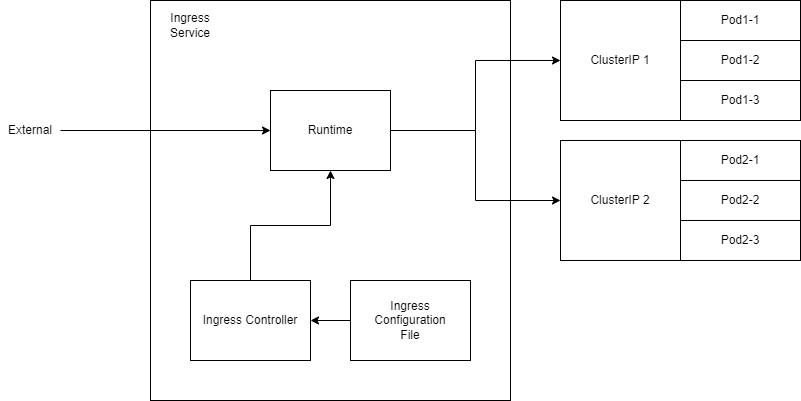
\includegraphics[width=350pt]{chapters/part-3/figures/ingress_service.png}
	\caption{An example of ingress service framework.} \label{ch:vac:fig:ingress_service}
\end{figure}

The ingress configuration differs depending on the ingress service type and the platform. Details are not given here.

\subsection{Volumes} \label{ch:vac:subsec:k8svolume}

Docker engine uses volumes to maintain persistent data and share data among containers. Details have been introduced in Section \ref{ch:vac:subsec:dockervolume}. Kubernetes volume framework is similar in the sense that it makes sure that the data is saved and managed by the host machine, so that when the pods or containers are shutdown or restarted, the data can be restored safely.

Do notice that when comes to data sharing using volume, it is dangerous to have multiple containers or the host machine accessing the same files simultaneously, without knowing the existence of each other. Usually additional steps need to be setup to ensure data consistency.

It is worth emphasizing the differences of ``volume'' technology in containerization and Kubernetes volume-related objects: Persistent Volume Claim (PVC). Persistent Volume (PV), and Volume. As a matter of fact, Kubernetes Volume object is usually not what we want. Kubernetes Volume creates the volume tied to a pod, not to the host machine. It survives container failure in the pod, but not pod failure. In summary:
\begin{itemize}
	\item Kubernetes Volume: A volume tied to the pod. It survives container failure inside the pod, but not pod failure.
	\item Kubernetes PV: A volume tied to the host machine. It survives pod failure. It can be provisioned either automatically by a StorageClass, or manually by the developer and administrator.
	\item Kubernetes PVC: It is essentially a request sent from a pod or a container, asking for specific amount of storage from a PV. Kubernetes will find that amount of PV from either existing provisioned static PV, or dynamically provision new ones for the pod or container.
\end{itemize}
Notice that it is not necessary to claim PV in order to use PVC, as PVC can provision PV dynamically. There is a one-to-one relationship between the provisioned PV and the PVC. If there are multiple pods, each requiring a dedicated PV, then multiple PVCs must be used. The developer can either create those PVCs manually, or use a Volume Claim Template to claim them if they are similar.

An example of claiming Kubernetes PV and PVC is given below. In the remaining part of this section, we will be mostly using PVC instead of PV.
\begin{lstlisting}
# persistent-volume.yaml

apiVersion: v1
kind: PersistentVolume
metadata:
name: my-pv
spec:
storageClassName: standard
capacity:
storage: 10Gi
accessModes:
- ReadWriteOnce
hostPath:
path: /data/my-pv
---
# persistent-volume-claim.yaml

apiVersion: v1
kind: PersistentVolumeClaim
metadata:
name: my-pvc
spec:
storageClassName: standard
accessModes:
- ReadWriteOnce
resources:
requests:
storage: 5Gi
\end{lstlisting}
To check the PV objects, use \verb|$ kubectl get pv| and \verb|$ kubectl get pvc|.

To add the above Kubernetes PVC to a Kubernetes Deployment, add volumes information to the specs as given in the following example.
\begin{lstlisting}
apiVersion: apps/v1
kind: Deployment
metadata:
name: my-app-deployment
spec:
replicas: 1
selector:
matchLabels:
app: my-app
template:
metadata:
labels:
app: my-app
spec:
containers:
- name: my-app-container
image: my-app-image
ports:
- containerPort: 8080
volumeMounts:
- name: data-volume
mountPath: /data
subPath: data-from-container
volumes:
- name: data-volume
persistentVolumeClaim:
claimName: my-pvc
\end{lstlisting}
where \verb|volumes| defines which Kubernetes PVC is used, and \verb|volumeMounts| tells how it is mounted in the container. The \verb|mountPath| is the path in the container whose data is mounted by the volume. If a \verb|subPath| is given, a sub-folder of its specified name will be created in the host machine in the volume to contain the data.

There are different types of access modes:
\begin{itemize}
	\item \verb|ReadWriteOnce|: Allow one node to read and write at a time.
	\item \verb|ReadOnlyMany|: Allow many nodes to read at a time.
	\item \verb|ReadWriteMany|: Allow many nodes to read and write at a time.
\end{itemize}

The developer can specify the place for Kubernetes PVs. This is usually the hard drive on a local server, a virtual storage space in the VM. Use the following command to check Kubernetes possible choice of storage.
\begin{lstlisting}
	$ kubectl get storageclass
\end{lstlisting}
and
\begin{lstlisting}
$ kubectl describe storageclass
\end{lstlisting}
When deploying Kubernetes on the Cloud, the developer needs to do additional configurations as there would be many storage options. Usually, each Cloud provider will have its own default storage space for Kubernetes, such as AWS Elastic Block Store for AWS.

\subsection{Secrets} \label{ch:vac:subsec:k8ssecrets}

Kubernetes Secrets object is used store confidential information, such as the database password, API key, etc. It is often a piece of information that is necessary for the containers, but the developer does not want to present as plain text in the configuration file.

Secrets are not created from configuration files, which is the recommended way of creating other Kubernetes objects. Instead, it is created from one-time imperative command, inside which the confidential information needs to be told to Kubernetes. Use the following command to create a Secret object.
\begin{lstlisting}
$ kubectl create secret <type-of-secret> <secret-name> --from-literal <key>=<value>
\end{lstlisting}
There are 3 types of Secrets: \verb|generic|, \verb|docker-registry| and \verb|tls|.

\subsection{Kubernetes Environment Variables}

Kubernetes environment variables are used to pass or share information among Deployments. Depending on the features of the information, such as whether it is a constant global configuration or a dynamic value, whether it is plain text or confidential encoding, etc., it might be handled differently.

To define constant environment variables in containers, simply specify them in the Deployment configuration file as given in the example below.

\begin{lstlisting}
apiVersion: apps/v1
kind: Deployment
metadata:
name: my-app-deployment
spec:
replicas: 1
selector:
matchLabels:
app: my-app
template:
metadata:
labels:
app: my-app
spec:
containers:
- name: my-app-container
image: my-app-image
ports:
- containerPort: 8080
volumeMounts:
- name: data-volume
mountPath: /data
subPath: data-from-container
env:
- name: <name1>
value: <value1>
- name: <name2>
value: <value2>
- name: <name3>
valueFrom:
secretKeyRef:
name: <secret-name>
key: <key>
volumes:
- name: data-volume
persistentVolumeClaim:
claimName: my-pvc
\end{lstlisting}
where a new tag \verb|env| is defined under template, specifications, containers. Under the \verb|env| tag, a list is defined containing names and values of the environment variables. The value must be a string, not a numerical number.

\section{Kubernetes Deployment in Production Environment}

With the tools and methodologies introduced so far, we are able to deploy containers in development environment. This is good enough for testing purpose or for small individual projects. However, when comes to enterprise tier projects or collaborative projects, there is often a CI/CD pipeline that standardize the integration and delivery of the containers in production environment. Container orchestration tools such as Kubernetes is often a must have.

This section briefly introduces the steps to develop and deploy containers in production environment with Kubernetes. Figure \ref{ch:vac:fig:prodenvworkflow} gives an example of overview of what such deployment may look like. Notice that this example is more towards a community project but not an enterprise project.

\begin{figure}[htbp]
	\centering
	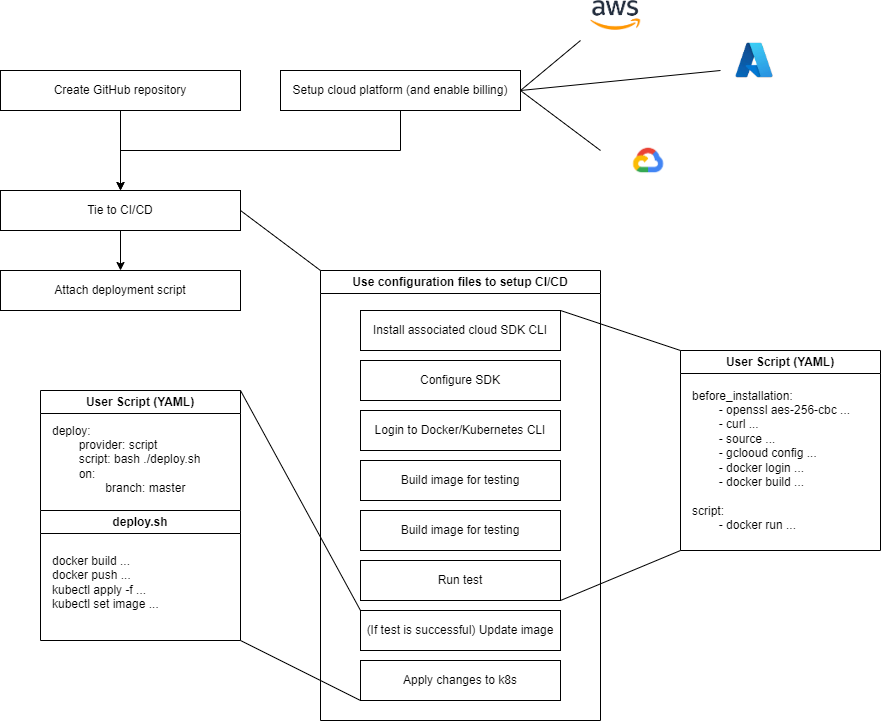
\includegraphics[width=350pt]{chapters/part-3/figures/prodenvworkflow.png}
	\caption{An example workflow of creating a production environment with Kubernetes.} \label{ch:vac:fig:prodenvworkflow}
\end{figure}

The example used in this section to demonstrate Kubernetes CI/CD on a cloud platform in production environment is taken from \cite{stephen2023docker}. Following \cite{stephen2023docker}, Google Cloud Platform is used as the cloud platform provider.

\subsection{Setup Cloud Account}

Many cloud platforms nowadays have a very good support of Kubernetes. The deployment of containers using Kubernetes can be done via their UIs easily. The developer needs to decide the resources to be used for the deployment. The more nodes and more power machine, the higher the charge. In most cases, the developer does not need to start a VM and install Kubernetes on it by himself. The cloud provider shall have dedicated Kubernetes engine service that would automatically configure the VM per required.

\subsection{Configure CI/CD}

Travis CI is a continuous integration service tool written. It can be deployed on the cloud and linked to a Github repository and a CI/CD platform such as a Kubernetes cluster on Google Cloud Platform.

To run Travis, a machine supporting Ruby programming language is required. For that, a separate container with Ruby installation is deployed to run Travis. Use Github credentials to login to Travis, so that it can link to the Github repositories.

Travis has built-in file encryption function. This function is mainly used to encrypt login credentials and service account credentials (in this example, the service account information to link to Kubernetes clusters on Google Cloud Platform) locally, so that later the unencrypted original credential files can be deleted, and only the encrypted credentials uploaded to the Github repository. When encrypting a file, Travis will also guide the user on how to call the encrypt information in the build script.

Travis uses configuration files to setup CI/CD pipeline.

\subsection{Deploy Containers}

In the Travis configuration file, \verb|deploy| is used to specify the script to run when the testing is successful. A separate bash script \verb|deploy.sh| is defined for this purpose, inside which is a sequence of commands that builds and publishes images, and configures Kubernetes using \textit{kubectl}.

It is particularly worth mention that in \verb|deploy.sh|, when building and applying the latest version of the docker image, tagging using \verb|<image-name>:latest| alone is not going to work. This is because when the same configuration with \verb|<image-name>:latest| is applied, the system would simply acknowledge it as ``no change'' and would not actually download the latest version of the image.

The walk introduced earlier was to use version number in the configuration file and/or as an imperial command as follows.
\begin{lstlisting}
$ kubectl set image deployment/<Deployment name> <container name>=<image name>:<version>
\end{lstlisting}
so what when the version name changes, Kubernetes would notice the differences and apply the new image. When working with CI/CD using \textit{Git}, this can be further automated. Just use the \verb|$GIT_SHA| as part of the tag as follows.
\begin{lstlisting}
$ docker build -t <docker-id>/<image-name>:latest -t <docker-id>/<image-name>:$GIT_SHA -f <dockerfile> <save-directory>
$ docker push <docker-id>/<image-name>:latest
$ docker push <docker-id>/<image-name>:$GIT_SHA
\end{lstlisting}
Notice that in addition to \verb|:latest|, \verb|:$GIT_SHA| is used as a secondary tag. When pushing the built image to Docker Hub, both \verb|:latest| and \verb|:$GIT_SHA| are pushed (although they have identical content). When setting image, the \verb|$GIT_SHA| is used to identify the image just like the version number.

It is recommended not to remove \verb|:latest| in the building command. This is because if someone wants to pull and test the latest image in his server (without knowing the value of \verb|$GIT_SHA| for the latest commit), he is still able to do so using only the image name.

Notice that \verb|$GIT_SHA| is not a built-in environment variable. The developer needs to set that environmental variable manually in the configuration YAML file as follows. It is possible to replace \verb|$GIT_SHA| with a different name.
\begin{lstlisting}
env:
global:
- GIT_SHA=$(git rev-parse HEAD)
\end{lstlisting}
With the above setup, \verb|$GIT_SHA| can be used in \verb|deploy.sh| as an environmental variable.

\subsection{Manage Secrets}

Notice that when CI/CD tool is tied to the cloud platform provider, service account authentication is required. It is a good habit to NOT to put the authentication information in the CI/CD configuration file as plain text, or to upload the unencrypted file that contains the authentication information to the public workspace. It is possible that some CI/CD tools provide encryption tools that can be used to encrypt the authentication file. In such case, the developer may need to install the required CLI for that CI/CD tool.

In Section \ref{ch:vac:subsec:k8ssecrets}, it has been introduced that Kubernetes uses Secrets object to encrypt secret files. The encrypted secret files can then be safely published online. In the Kubernetes configuration file, an environmental variable can be created to call the secret information.

Many cloud platform providers including Google Cloud Platform provides services to manage secrets.

\subsection{Helm}

To install a software in a Kubernetes pod, the most intuitive way is to commit the installation in the image, and call the image in the Kubernetes configuration file. For commonly used services such as \verb|ingress-nginx|, its installation configuration file is available online as part of the manual. It essentially starts and initializes a branch of Kubernetes objects to enable the service.

Helm is designed as an alternative to manage software installation in Kubernetes clusters. In many occasions, it is more convenient (or even only possible) to use Helm to install a software. More details are given in \textit{github.com/helm/helm}.

We need to first install Helm from script. Helm installation used to contain two parts, the CLI (referred as Helm client) and the server (referred as Tiller server). We could then use Helm CLI to install other third-party software and tools.

Access control is important on cloud platforms. In practice, user accounts are used to identify users, and service accounts to identify pods and programs. Associated role bindings are used to manage what resources can be accessed by a user or program. For example, administrative role over the entire account can be used to bind with the administrative user. The same applies to Helm. The Tiller server required some extent of administrative control over the resources in an account. In many occasions, Tiller server was given the administrative permission to access the entire account, which introduced security risks.

As of Helm version 3, a major change was carried out where Tiller server was removed completely. Helm architecture is more secure and simpler today. The concerns related to Tiller's permission in the Kubernetes cluster are no longer relevant. Helm 3 of course requires permissions to use the resources, which is now managed by Kubernetes role-based access control mechanisms.

\section{Alternatives to Kubernetes}

Portainer is an open-source container orchestrator that has a user-friendly interface and is relatively easier to use than the more powerful and famous container orchestrator Kubernetes which is introduced in the next chapter. In this section, it is used as an example, just to give the reader an idea what container orchestrators in the market may look like. The section does not go into details about Portainer.

Before starting a Portainer container, it is a good practice to first create a docker volume for Portainer to store the database. Use the following command to create such docker volume.
\begin{lstlisting}
$ docker volume create portainer_data
\end{lstlisting}
Then run a Portainer container using
\begin{lstlisting}
$ docker run -d -p 8000:8000 -p 9000:9000 -p 9443:9443 --name portainer --restart=always -v /var/run/docker.sock:/var/run/docker.sock -v portainer_data:/data portainer/portainer-ce
\end{lstlisting}
where ports 8000, 9000 and 9443 are used for hosting HTTP traffic in development environments, hosting web interface, and hosting HTTPS or SSL-secured services, respectively. The \verb|docker.sock| is the socket that enables the docker server-side daemon to communicate with its command-line interface. The image name for Portainer community edition (distinguished form the business edition) is \verb|portainer/portainer-ce|.

Use \verb|https://localhost:9443| to login to the container. The following page in Fig. \ref{ch:vac:fig:portainerlogin} should pop up in the first-time login, asking the user to create and administration user.
\begin{figure}[htbp]
	\centering
	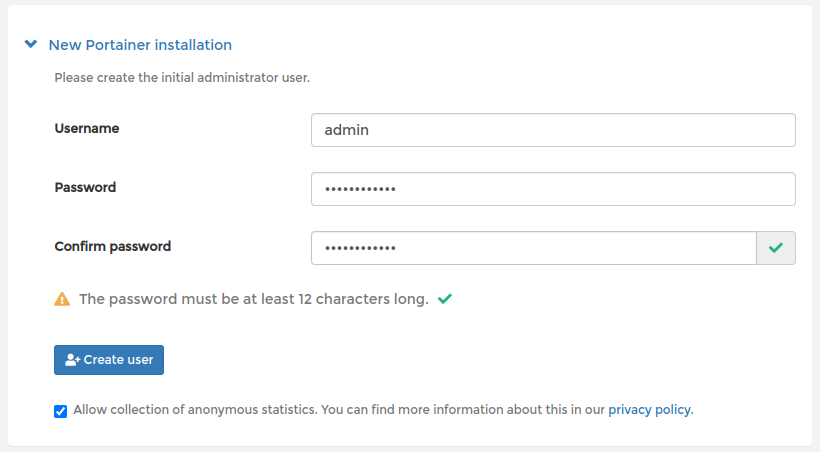
\includegraphics[width=350pt]{chapters/part-3/figures/portainerlogin.png}
	\caption{Portainer login page to create admin user.} \label{ch:vac:fig:portainerlogin}
\end{figure}

After creating the admin user and logging in, the status of images, containers and many more can be monitored via the dashboard, as shown in Figs. \ref{ch:vac:fig:portainerdashboard1}, \ref{ch:vac:fig:portainerdashboard2} and \ref{ch:vac:fig:portainerdashboard3}. Notice that in Fig. \ref{ch:vac:fig:portainerdashboard3}, using the ``quick action'' buttons, the user can check the specifics of the container and interact with its console, just like using \verb|docker container inspect| and \verb|docker exec|
\begin{figure}[htbp]
	\centering
	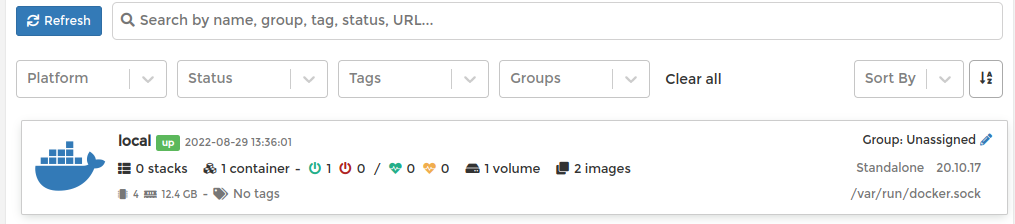
\includegraphics[width=350pt]{chapters/part-3/figures/portainerdashboard1.png}
	\caption{Portainer dashboard overview of docker servers.} \label{ch:vac:fig:portainerdashboard1}
\end{figure}

\begin{figure}[htbp]
	\centering
	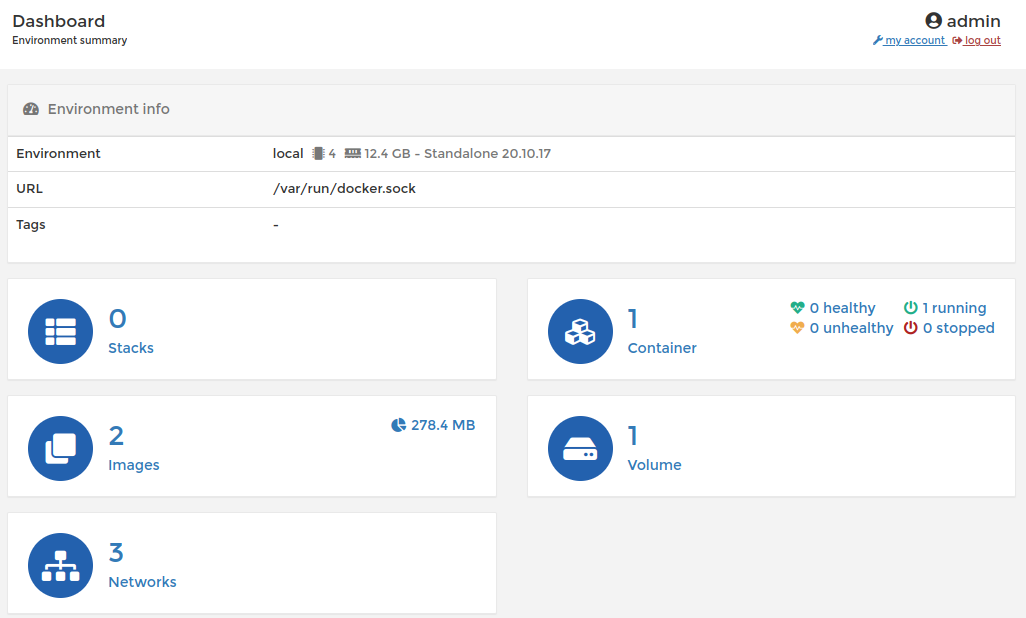
\includegraphics[width=350pt]{chapters/part-3/figures/portainerdashboard2.png}
	\caption{Portainer dashboard overview in a docker server.} \label{ch:vac:fig:portainerdashboard2}
\end{figure}

\begin{figure}[htbp]
	\centering
	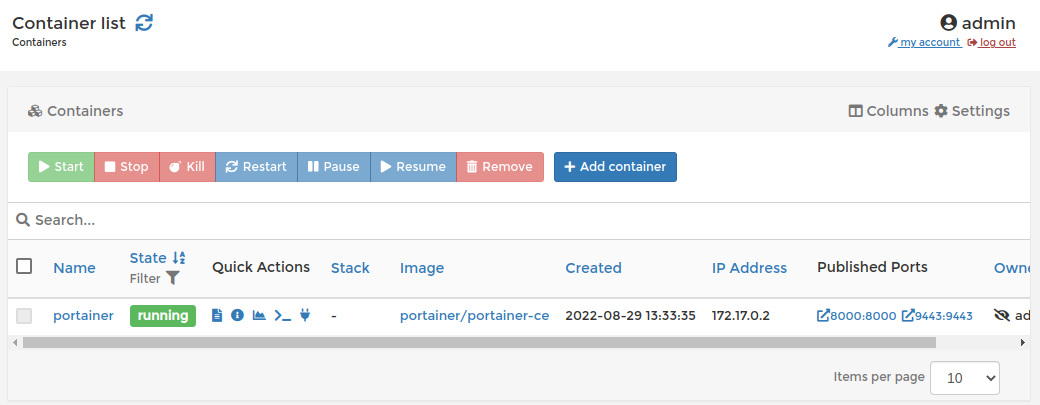
\includegraphics[width=350pt]{chapters/part-3/figures/portainerdashboard3.png}
	\caption{Portainer dashboard list down of all running containers.} \label{ch:vac:fig:portainerdashboard3}
\end{figure}

In summary, Portainer is an easy-to-use container management tool with clean graphical interface that a user can quickly get used to without a steep learning curve. 